    \chapter{Estudo de caso e metodologia}
%\addcontentsline{toc}{chapter}{Estudo de caso e metodologia}
        Esta sessão descreve o dispositivo a ser testado, assim também como a metodologia utilizada para abordar a modelagem de software.



\section{O dispositivo sob teste e sua jiga}

        Como mencionado no capítulo \ref{intro}, o escopo de desenvolvimento foi reduzido a um único produto como forma de simplificação de projeto. Considerando isto, escolheu-se o GT650\footnote{\citep{v2com2016}}, que é o produto principal da empresa. Projetado para atender demandas de distribuição de energia, o GT650 é um módulo de comunicação móvel para gerenciamento de medições automatizadas controle de redes de transmissão e distribuição. Sua PCIM pode ser vista nas figuras \ref{fig:board} e \ref{fig:board_inf}.
        
        \begin{figure}
            \centering
            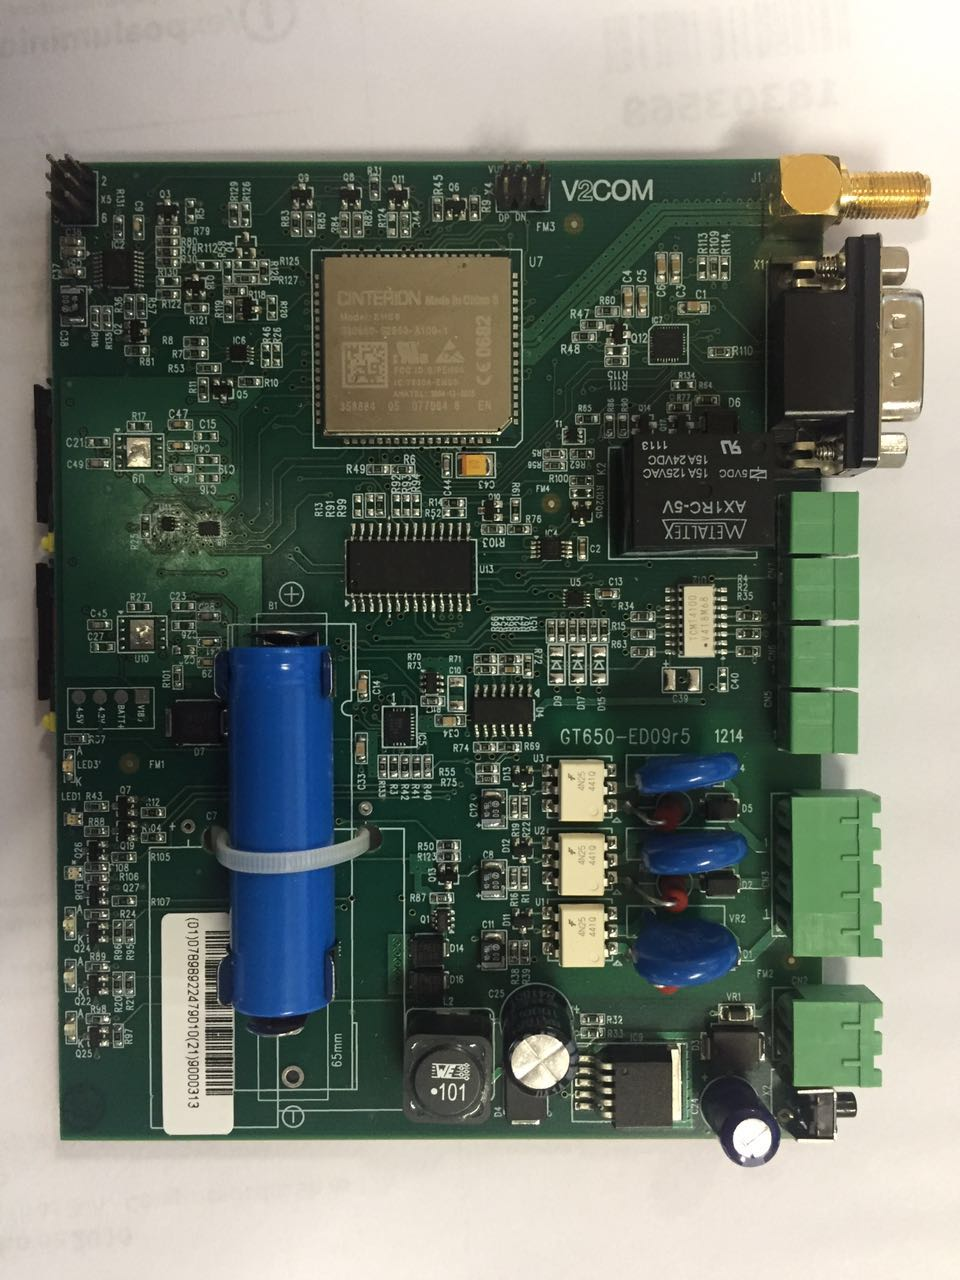
\includegraphics[width=0.9\linewidth]{board}
            \caption{foto do lado superior  do GT650}
            \label{fig:board}
        \end{figure}
        
        \begin{figure}
            \centering
            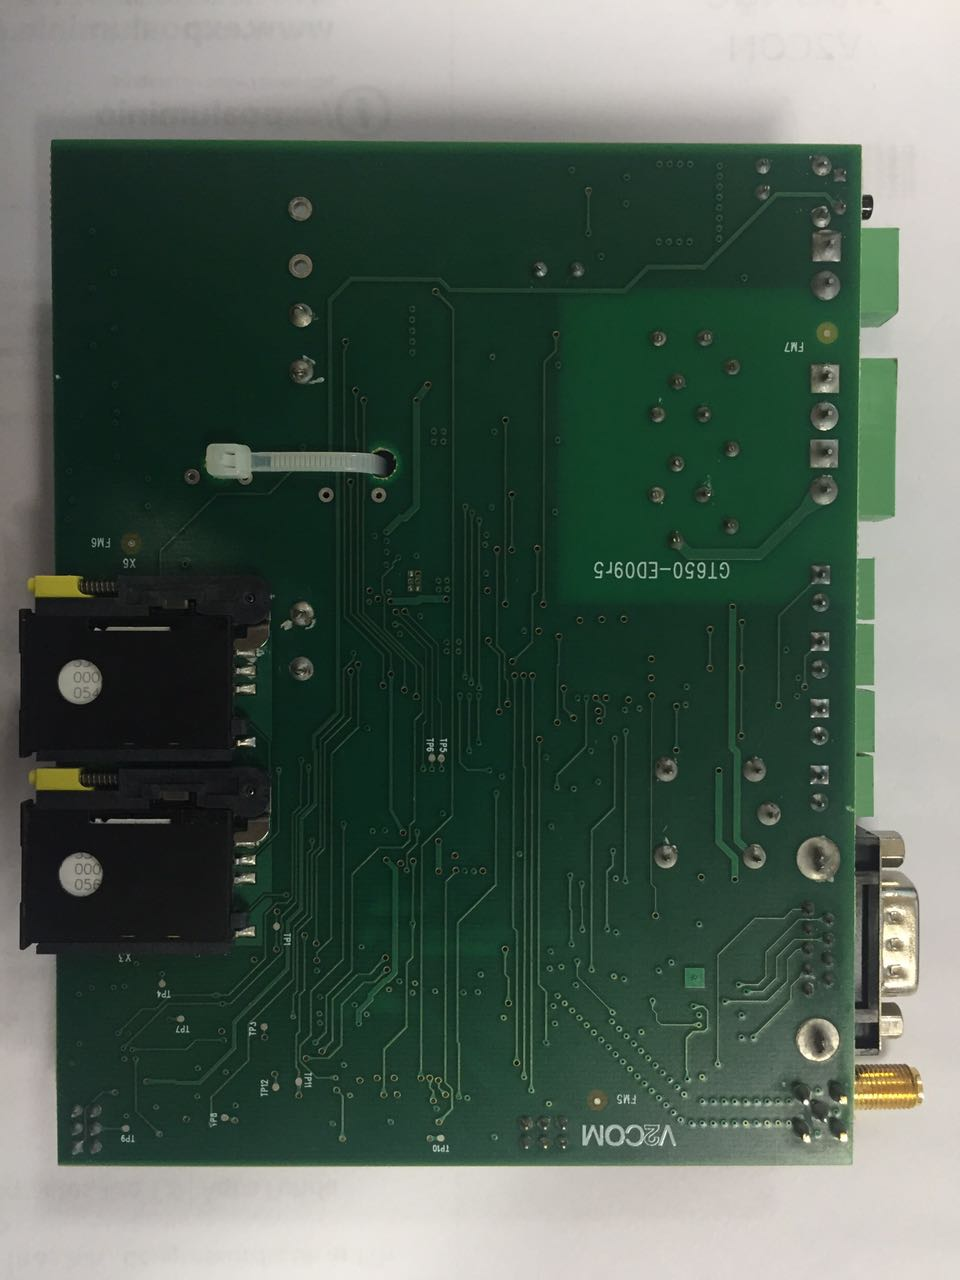
\includegraphics[width=0.9\linewidth]{board_under}
            \caption{foto do lado inferior  do GT650}
            \label{fig:board_inf}
        \end{figure}
        
        Segundo o site da empresa, o GT650 serve como um módulo integrável à qualquer religador, medidor de energia, ou dispositivo de distribuição, por diversos protocolos, sendo RS-232 e Ethernet os mais utilizados. 
        Seu software embarcado pode ser atualizado remotamente via OTAP (over-the-air provisioning\footnote{over-the-air provisioning é um método de atualização de software remotamente. Isso é normalmente implementado no próprio bootloader do sistema \citep{jacobbeningo2013}.}) e sua operação continua é assegurada por uma bateria de lítio embutida. Além disso o módulo possui sensor de tensão trifásica para detecção de anormalidades, e portas digitais para detectar a abertura de gabinetes ou qualquer outra customização que o cliente solicitar.
        
        \begin{figure}
            \centering
            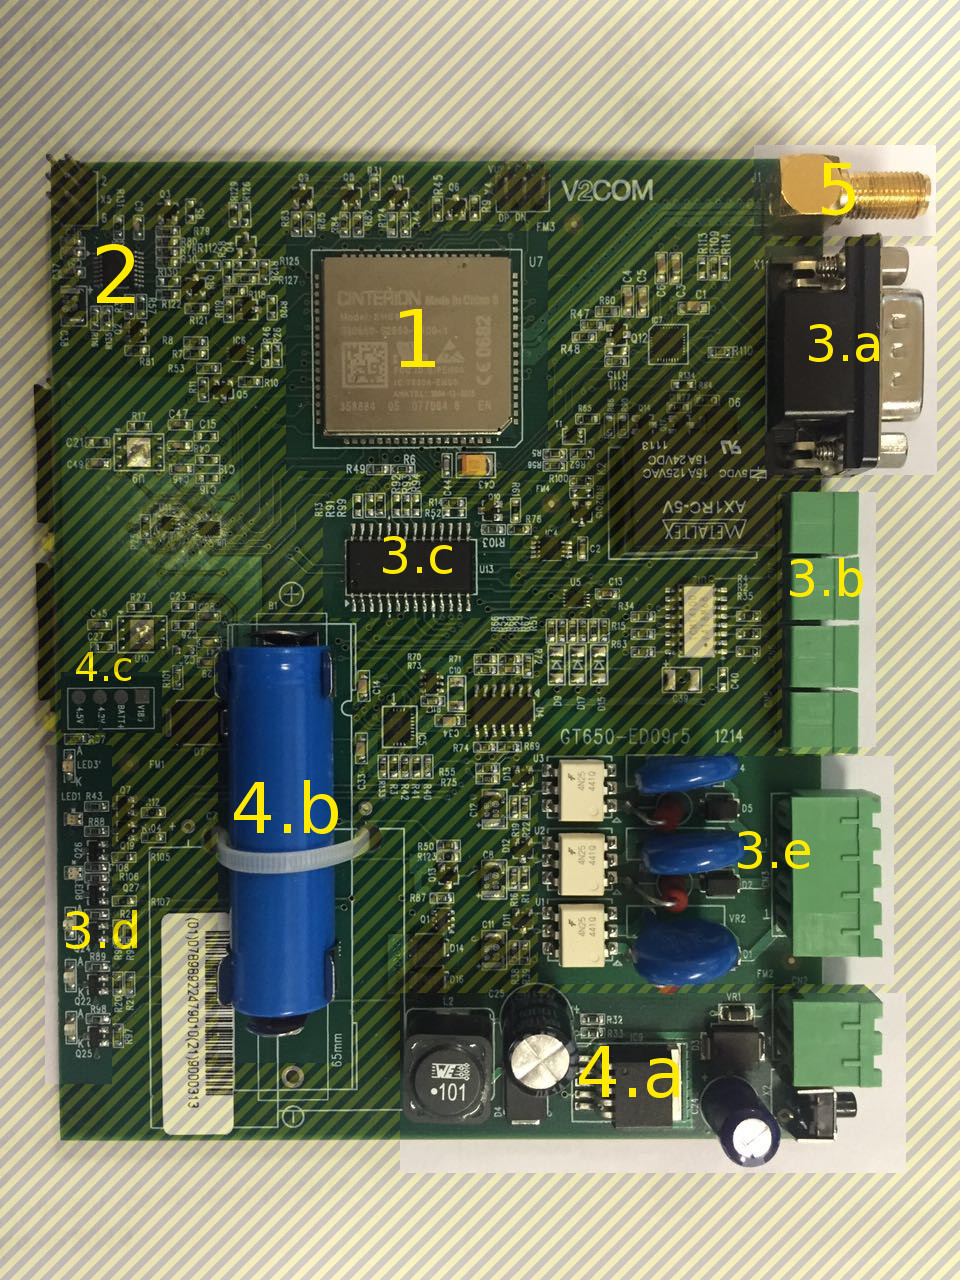
\includegraphics[width=0.9\linewidth]{placa}
            \caption{foto do GT650 com destaque aos componentes da placa}
            \label{fig:placa}
        \end{figure}
        
            \subsubsection{Módulo M2M}
                O processador principal da placa é o modem EHS6 da  Cinterion (ponto 1 da figura \ref{fig:placa}), que segundo o site do fabricante, contém: %todo cite EHS6 DATASHEET
                
                \begin{itemize}
                    \item Cinco bandas de 3G (HSPA): 800/850/900/1900/2100 MHz
                    \item Quatro bandas GPRS/EDGE Class 12: 850/900/1800/1900 MHz
                    \item Suporte a Java™ ME\footnote{Java Micro Edition é  uma plataforma Java para sistemas embarcados} 3.2, com suporte a multi-threading e execução de múltiplas aplicações, além de 6 MB de memória RAM e 10 MB de memória Flash;  %todo cite JAVA ME
                    \item Pilha de protocolos TCP/IP embarcada e acessível por comandos AT, incluindo conexão segura via TLS/SSL; serviços DNS e Ping; Cliente FTP e HTTP; %todo cite AT Commands
                    \item Interface USB 2.0 HS, e duas portas de interface modem serial;
                    \item 16 GPIOs compartilhadas com as portas de comunicação, PWM, etc.
                    \item ADC e interface I$^{2}$C 
                    \item Atualização de \textit{Firmware Over-the-air} (FOTA)
                \end{itemize}
                
                Basicamente é o componente central do produto: Comunicação TCP/IP via GSM/3GPP/GPRS; Aplicações Java, interface serial com o mundo externo e I$^{2}$C com os componentes periféricos da placa.
                
                O fabricante não fornece informações internas sobre a arquitetura, como também nenhum meio de acesso à estrutura interna do módulo. Como contrapartida a empresa oferece garantia de funcionamento, assim como suporte técnico completo.
                
                Todavia, isto impede testes estruturais e verificações mais profundas nos módulos, tanto na produção, quanto na manutenção e torna todos os processos dependentes de agentes externos. O teste estrutural se limita a verificação de interconexões do componente com a placa. Como já mencionado este teste é realizado pela empresa responsável pela montagem e é realizado através de equipamentos de AXI -- \textit{caso a contratada possua} -- Pois o encapsulamento LGA impossibilita conferir visualmente, ou por AOI, todas as interconexões. 
                
                Todo e qualquer problema que ocorrer com estes módulos, seja físico ou de \textit{firmware}, é enviado ao fabricante original para solução, muitas vezes dependendo do suporte na Alemanha. Por um lado, é positivo já que tira da empresa, a responsabilidade de resolver problemas de baixo nível, assim como a necessidade de manter pessoal e equipamento especializado para analisar este tipo de problema. Por outro lado, trabalhar com componente e \textit{firmware} fechados deixa a produção sujeita a problemas invisíveis. Um erro de \textit{firmware}, por exemplo, poderia ocasionar um \textit{recall} de um lote inteiro.
                
                Por estas limitações no teste estrutural, o escopo de teste fica restrito às verificações funcionais, principalmente através de comandos AT, como veremos na sessão \ref{metodologia}. 
                
            \subsubsection{Monitor \textit{Watchdog}}
                Este componente é um microcontrolador simples de 8 bits (figura \ref{fig:placa}, no ponto 2), e é  responsável por desligar o modem por duas maneiras: a primeira pelo temporizador watchdog, e a segunda pelo botão liga-desliga. 
                
                Também é armazenado nele o número de série da placa. Dessa forma a empresa consegue separar o rastreamento dos \emph{modems} e das \emph{placas}, podendo intercambiá-las conforme necessário.
                
                No escopo de teste algumas coisas foram elencadas pela equipe: conferir o número de série, teste do botão liga-desliga, e teste do temporizador \textit{watchdog}.
                
            \subsubsection{Interfaces cabeadas e com o usuário}
                Por ser uma solução de comunicação para outros equipamentos, o GT650 não possui interfaces digitais e analógicas muito complexas, exceto pela comunicação de dados via GSM, que será descrita à parte. Como pode ser visto na figura \ref{fig:placa}, a placa possui:
                
                \begin{itemize}
                    \item Duas portas RS232 (\ref{fig:placa}-3.a);
                    \item Três portas de entrada digitais opto isoladas (\ref{fig:placa}-3.b); 
                    \item Um relé de saída (\ref{fig:placa}-3.b);
                    \item Seis LEDs de sinalização (\ref{fig:placa}-3.d);
                    \item Uma porta para conferência de tensão trifásica (\ref{fig:placa}-3.e);
                \end{itemize}
                
                Vale mencionar que as entradas e saídas digitais, assim como os LEDs são controlados pelo modem atrávés do expansor de GPIO (\ref{fig:placa}-3.c) por endereçamento I$^{2}$C.
                
                Assim como nos pontos anteriores o escopo de teste se limita a verificações funcionais.
                
            \subsubsection{Alimentação, bateria e BMS}
                O sistema de alimentação consiste em um conversor CC-CC de 12 Volts com saídas de 3.3 Volts e 5 Volts (figura \ref{fig:placa}-4.a), e uma bateria de lítio de 4.8 Volts para em caso de faltas na rede (figura \ref{fig:placa}-4.b). 
                
                Para testar este sistema, foram criados quatro pontos de teste na placa como vistos no ponto 4.c da figura \ref{fig:placa}: 5V, BATT+, 3V3, e 1.8V. Atualmente, o teste é realizado manualmente com o multímetro, ponto por ponto, mas enviando os dados de leitura pelas portas seriais de computador. Pretende-se automatizar esta etapa nas próximas revisões da jiga de testes.
                
            \subsubsection{Comunicação GPRS/EDGE/UMTS}
                A comunicação de dados por UMTS é a interface principal do módulo e opera nas bandas: 800, 850, 900, 1900 and 2100 MHz. Além disso suporta dois cartões SIM.
                
                Originalmente, este sistema era testado por um simples teste de comunicação, mas devido a problemas de queda de potência de sinal causados por solda mal feita, que só apareciam em campo, esta estratégia foi substituída. Atualmente é usado um medidor de potência RF -- O \emph{NI USB-5680} -- que tem uma faixa de frequência 50 MHz até 6 GHz, alcance de potência de -40 a +23 dBm, e uma banda de canal 10 a 100 MHz. Esta nova estratégia adotada, praticamente eliminou os retornos de campo por problemas de alcance do produto.

    \subsection{O que é testado e o que precisa ser testado}
        
        
        O roteiro de teste anterior a este trabalho consistia no teste sequencial das funcionalidades da placa, ou seja um teste funcional. Conforme mencionado na sessão anterior, pela própria ausência de uma porta JTAG ou outra forma de acesso interno, e também por não ter nenhuma lógica programável no produto, o teste estrutural se limita à verificação ótica ou radiográfica das interconexões das PCIM. 
        
        Neste trabalho, decidiu-se por reproduzir o mesmo roteiro de teste utilizado anteriormente para não causar impactos negativos na rotina da produção da empresa. 
        
        É importante notar que este roteiro é ainda bastante sequencial, abrindo a possibilidade de otimização com rotinas concorrentes no escopo de teste. Isto será descrito na sessão \ref{metodologia}, que trata da metodologia e especificação de software.
        
        
        %todo anexar roteiro anterior?

    \subsection{A Jiga de teste}
        
        A decisão da equipe de engenharia foi utilizar a jiga de testes corrente, e foi atribuído a um projetista de hardware da equipe a tarefa de especificar e desenvolver uma nova plataforma de teste. 
        
        Este foi um ponto considerado nas especificações do programa que serão vistas na seção \ref{metodologia} do presente trabalho. 
        
        Esta Jiga é basicamente testes de interface, não possuindo nenhuma ponta de teste ou algo que se aproxime de uma \emph{cama de pregos} de teste para testes mais internos.  
    
        A Jiga possui comunicação serial do DUT com o computador, assim como um ponto de conexão do aterramento da placa com o negativo do multímetro e sua comunicação serial com o PC. Também permite ao operador fixar níveis lógicos alto ou baixo nas portas digitais, assim como tensões trifásicas na porta trifásica.
    
    \section{Metodologia e especificação de Software} \label{metodologia}

    \subsection{Levantamento de Requisitos}
        Requisitos são objetivos ou restrições estabelecidas por clientes e usuários que definem as diversas propriedades do sistema. Os requisitos de software são, obviamente, aqueles dentre os requisitos do sistema que dizem respeito às propriedades de software. Tradicionalmente, eles são divididos em \textit{funcionais e não funcionais}.
        
        Requisitos funcionais são a descrição das funcionalidades que o programa deve oferecer. E é genérico no sentido que não necessariamente trata-se de interações com o usuário, mas também como funcionalidades ocultas como, por exemplo, uma API, interações com hardware, e comunicação \citep{bourque2014guide}.
        
        Requisitos não-funcionais são qualidades globais de um software como manutenibilidade, usabilidade, desempenho, custo e vários outros. Normalmente estes requisitos são descritos de maneira informal, de maneira controversa (certos objetivos são concorrentes um com o outro) e são difíceis de validar\citep{bourque2014guide}.
        
        A partir do cenário estudado anteriormente, foram levantados os seguintes requisitos não-funcionais:
        \begin{itemize}
            \item O programa deverá ser implementado em LabVIEW;
            \item Reusabilidade de código;
            \item Concorrência e paralelismo do roteiro de testes;
            \item Modularização dos testes e do roteiro;
            \item Interface de usuário ergonômica e intuitiva;
        \end{itemize}
        
        Já os requisitos funcionais consistem no roteiro de testes anterior a este trabalho, conforme decisão da equipe de engenharia de fábrica:
        \begin{itemize}
            \item Leitura e armazenamento do número de série colado na placa por um leitor de código de barras;
            \item Comunicação com o DUT via serial;
            \item Teste das duas portas seriais;
            \item Verificar se o modelo de modem é o EHS6;
            \item Verificar se a \textit{firmware} do modem é a mais atual;
            \item Armazenar o IMEI\footnote{\textit{International Mobile Station Equipment Identity} ou Identificação Internacional de Equipamento Móvel é um número de identificação global e único para cada telefone ou modem celular.} do modem;
            \item Configurar as GPIOs do modem conforme o perfil da aplicação;
            \item Abertura, seleção e teste das duas bandejas de cartão SIM\footnote{\textit{subscriber identity module}};
            \item Configurar e testar comunicação $I^{2}C$;
            \item Configurar operação do expansor de IO, MCP23018: interrupção espelhada, não incremento de ponteiro, interrupção push-pull;
            \item Configurar e testar do BQ24070, carregador de bateria e \textit{system power-path} do sistema;
            \item Teste de leitura da bateria;
            \item Teste do microcontrolador de watchdog (MC9S08QG8), e do botão liga e desliga;
            \item Leitura do número de série armazenado no MC9S08QG8, e validação deste com o número de série colado  na placa;
            \item Teste de comunicação e leitura do sensor de temperatura LM75
            \item Teste de morte de sessão;
            \item Testes dos barramentos de tensão da placa: 4.5V, 4.2V, BATT++, e 1.8V;
            \item Teste do painel de LEDs;
            \item Teste de detecção de retirada e inserção da fonte de alimentação;
            \item Teste das 3 portas digitais;
            \item Teste de acionamento e desarme de relé;
            \item Teste da porta de tensão trifásica - detecção de presença e ausência;
            \item Teste de interrupção de desligamento e reset da placa;
            \item Ainda que não presente no roteiro da linha de produção ( esta etapa é realizada posteriomente), possibilidade de teste de potência de sinal de transmissão HSPA;
            \item Geração de arquivos de log de teste em .txt;
            \item Notificação para o operador sobre sucesso ou falha do teste, assim como possibilidade de reteste.
        \end{itemize}
    Passado o levantamento de requisitos, a etapa seguinte foi a escolha de método de desenvolvimento, assim como as etapas do mesmo.
        
\begin{comment}
    \subsection{Workflow do projeto} % jeitinho de trabalhar
       
       Para a realização deste trabalho dentro da empresa, optou-se por um desenvolvimento incremental a partir de uma solução minimamente funcional. O projeto foi realizado em etapas, em ciclos curtos de desenvolvimento que pudessem ser entregues para receber a contrapartida da empresa e ser validado. Algo próximo da metodologia Agile. Esse processo permitiu uma maior interatividade entre as necessidades da aplicação, como forma de repensar a escopo do programa, e também facilitou o acompanhamento da gerência com o andamento do produto.
       
 %   \subsection{Síntese dos requisitos ambientais de teste}
% #todo

Validação do projeto
Controle de Qualidade
Melhorias de processos
Melhorias no produto
Auxilio na Manutenção
\end{comment}    